\begin{frame}\frametitle{Differential Cross Section. Plots}
\begin{figure}[htb]
  \begin{center}
   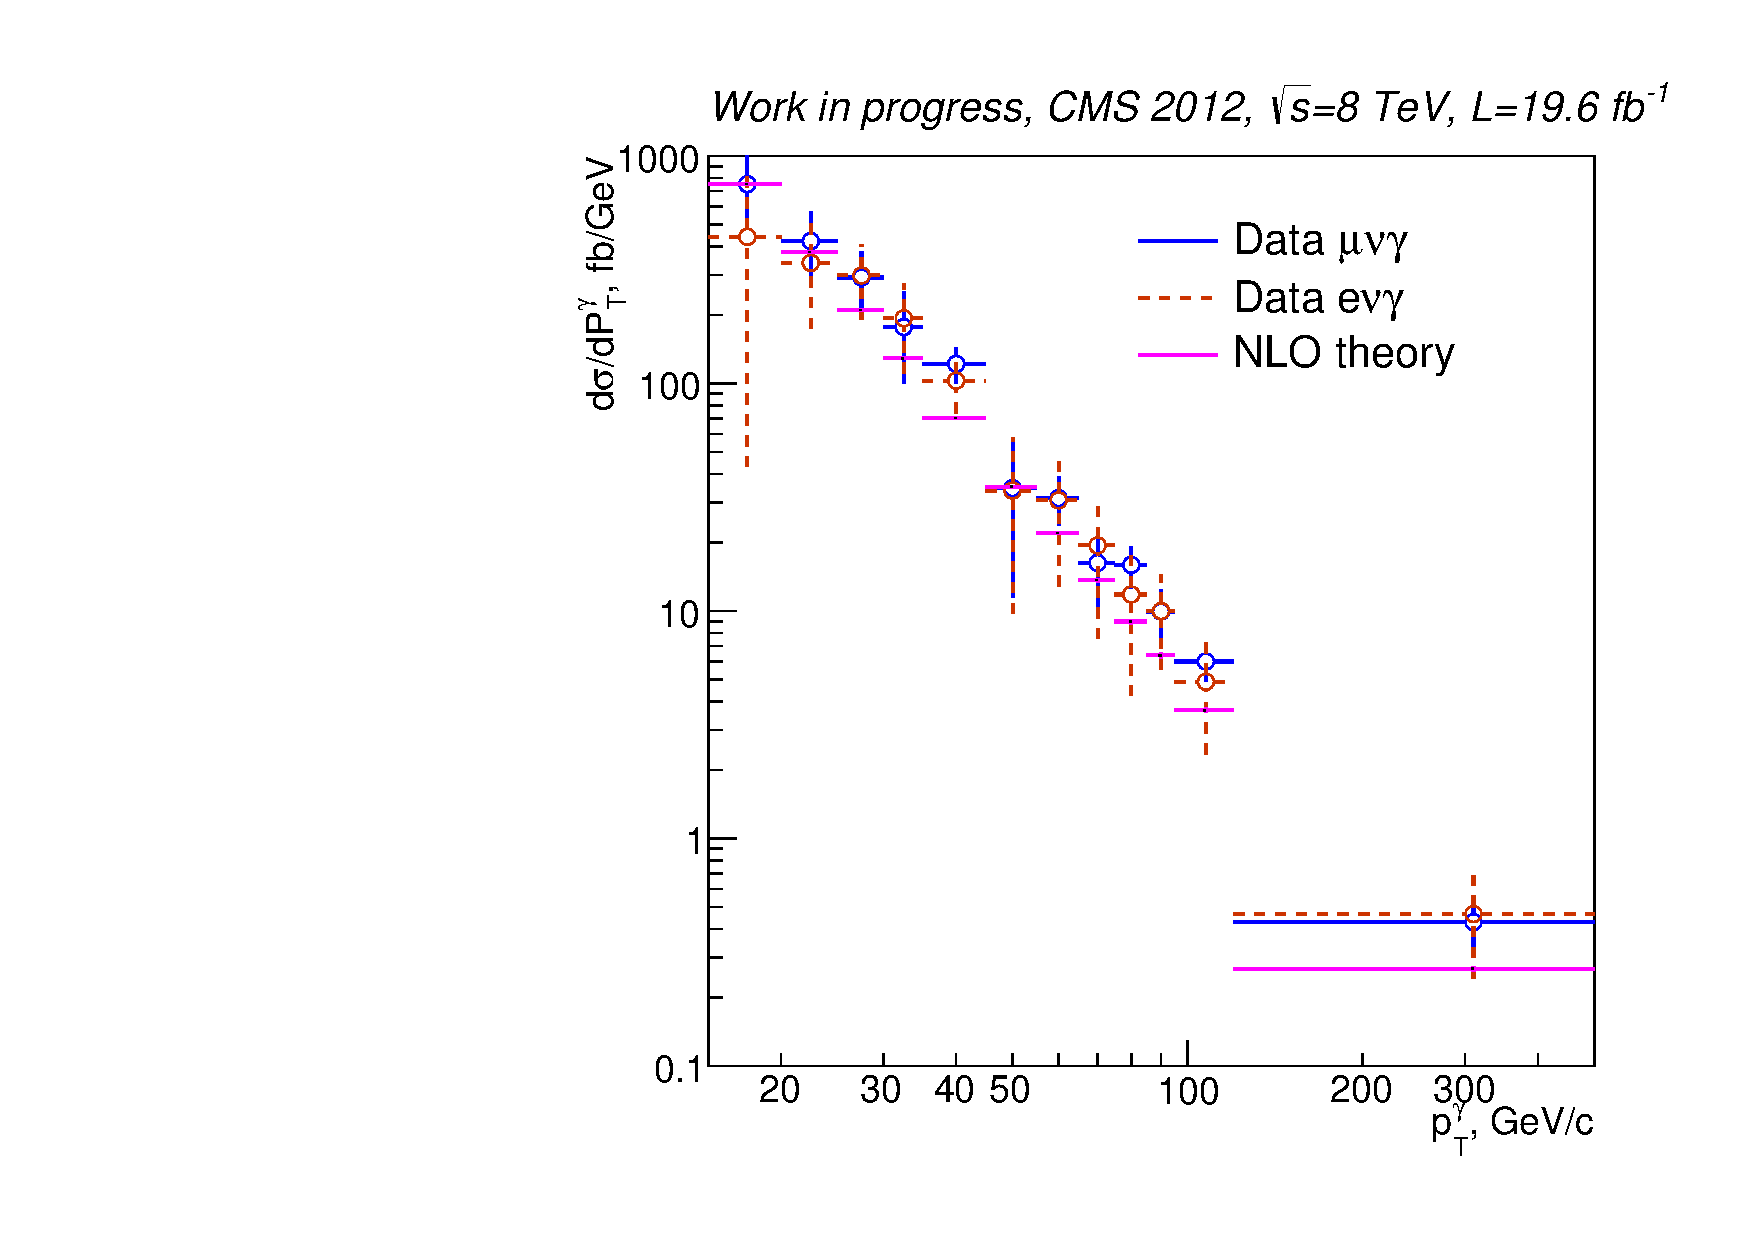
\includegraphics[width=0.5\textwidth]{../figs/figs_v11/ChannelsMERGED_WGamma/CrossSection/compareCSWGamma.pdf}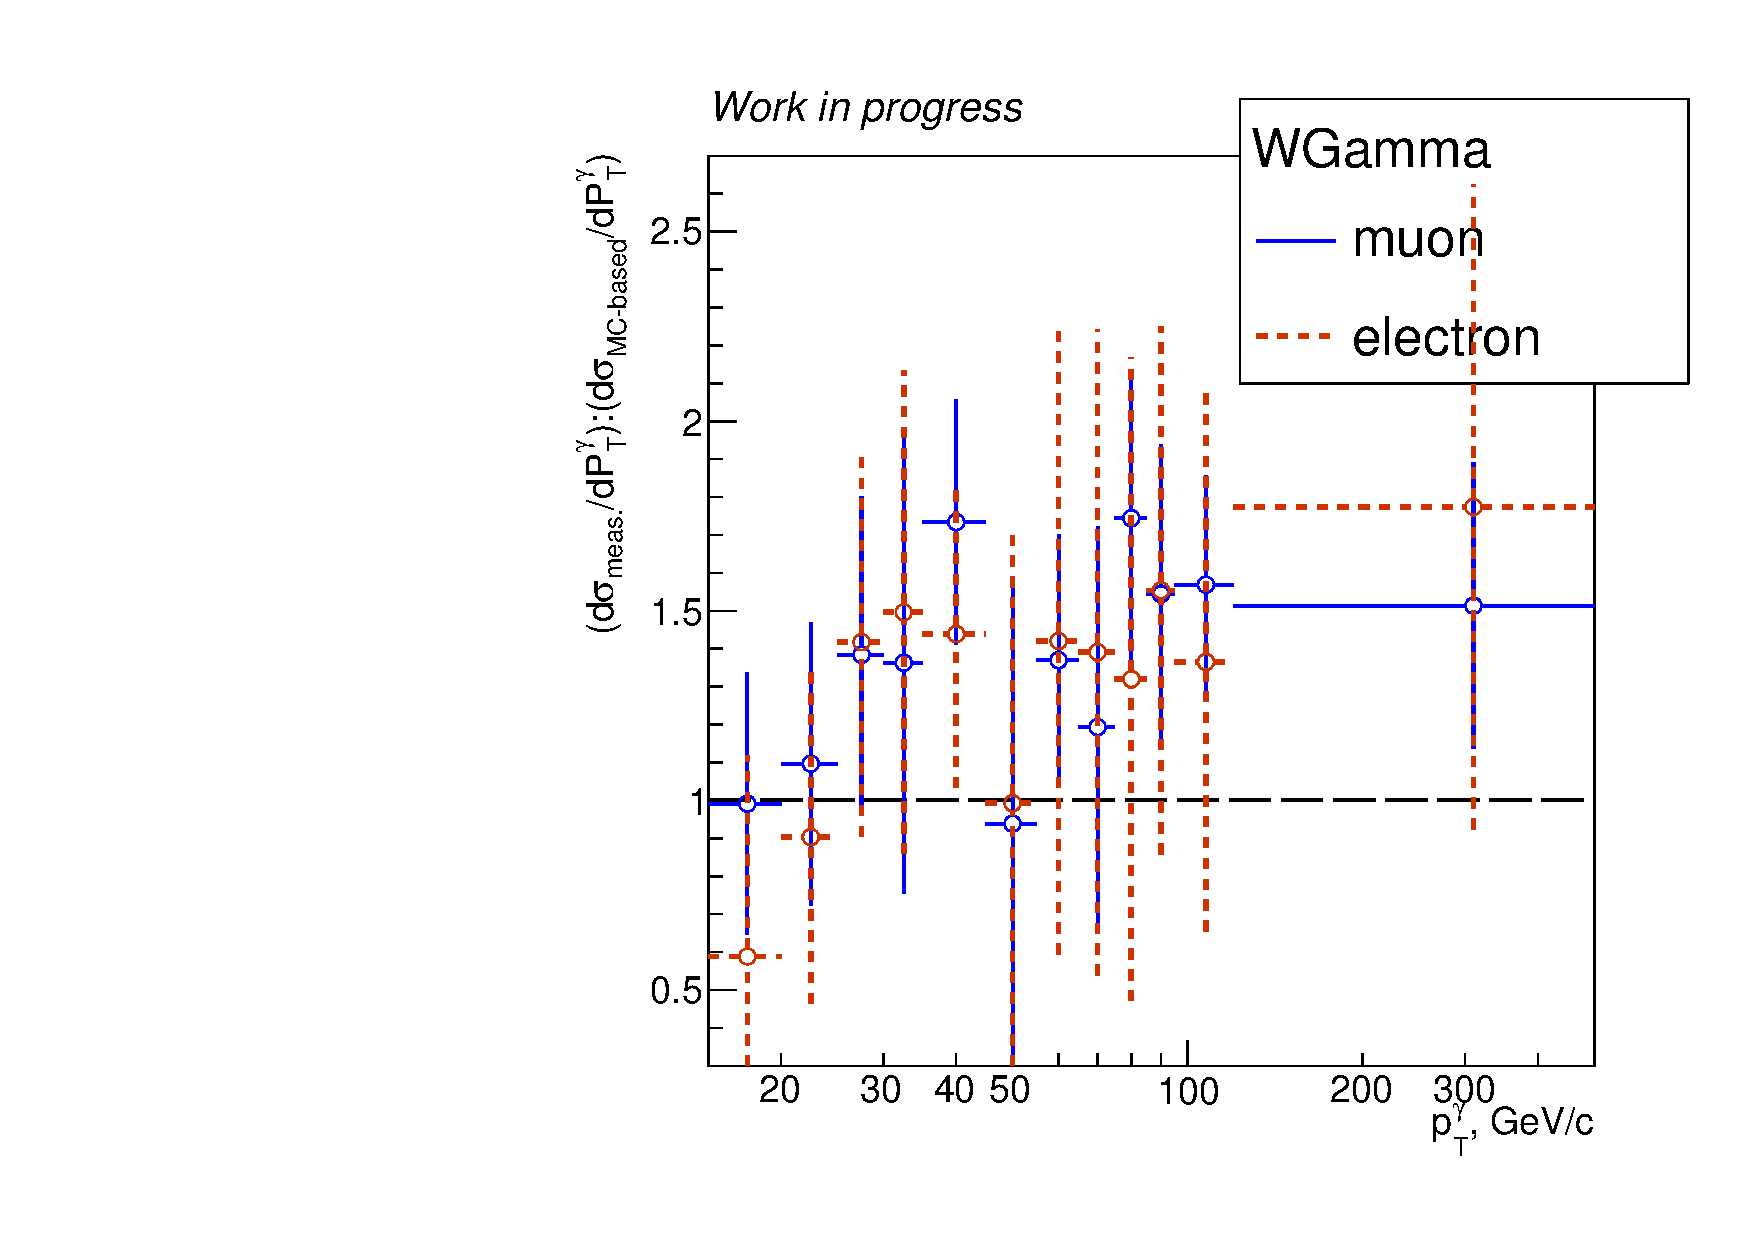
\includegraphics[width=0.5\textwidth]{../figs/figs_v11/ChannelsMERGED_WGamma/CrossSection/compareCSratioTheoryWGamma.pdf}\\
  \end{center}
\end{figure}
\scriptsize
{\bfseries{Total cross section ($P_T^{\gamma}>15$~GeV):}}\\
MC-based: $\sigma=9101$~fb\\
Measured, muon channel:   $\sigma = 10949 \pm 91 \pm 1463$~fb\\
Measured, electron channel:   $\sigma = 9146 \pm 185 \pm 2213$~fb\\
\end{frame}%{Differential Cross Section. Plots}

\begin{frame}\frametitle{ZGamma check. Differential Cross Section. Plots}
\begin{figure}[htb]
  \begin{center}
 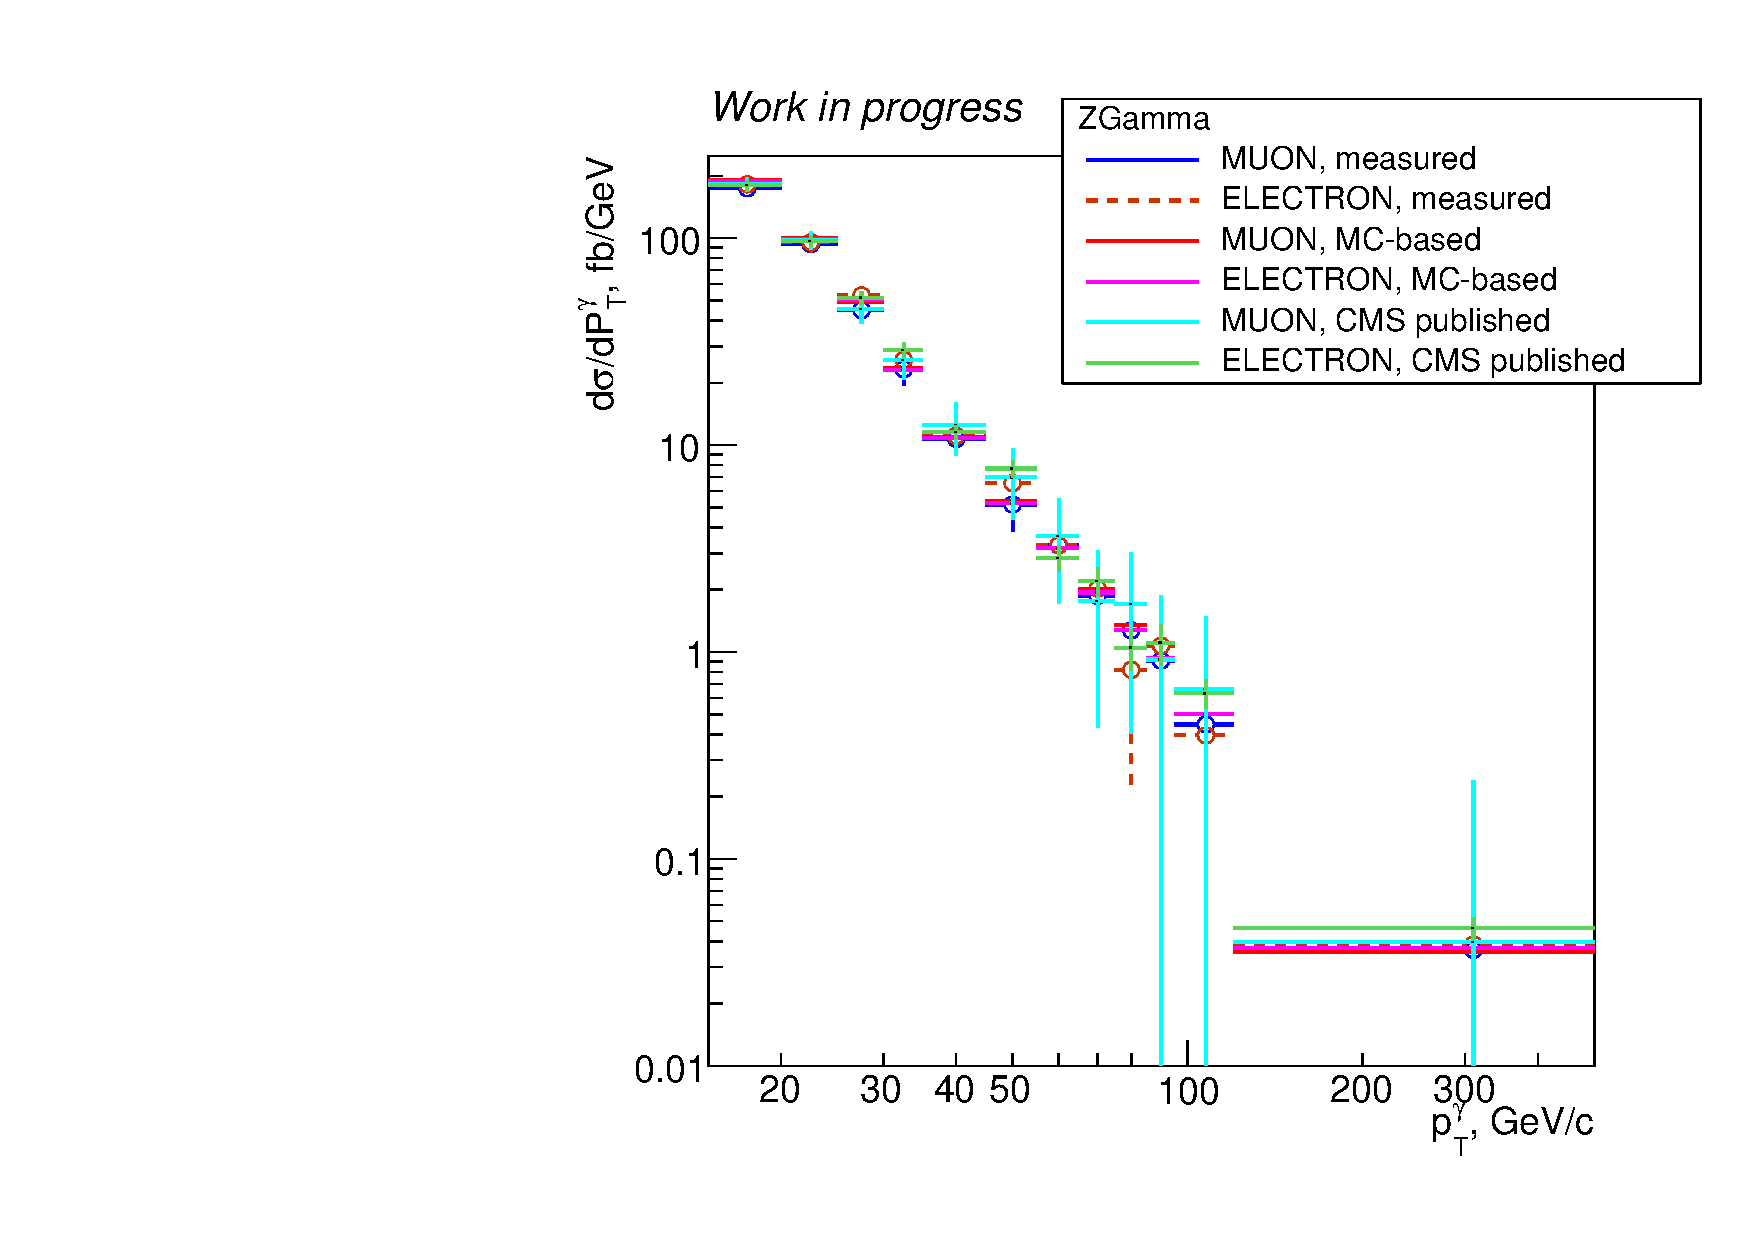
\includegraphics[width=0.45\textwidth]{../figs/figs_v11/ChannelsMERGED_ZGamma/CrossSection/compareCSZGamma.pdf}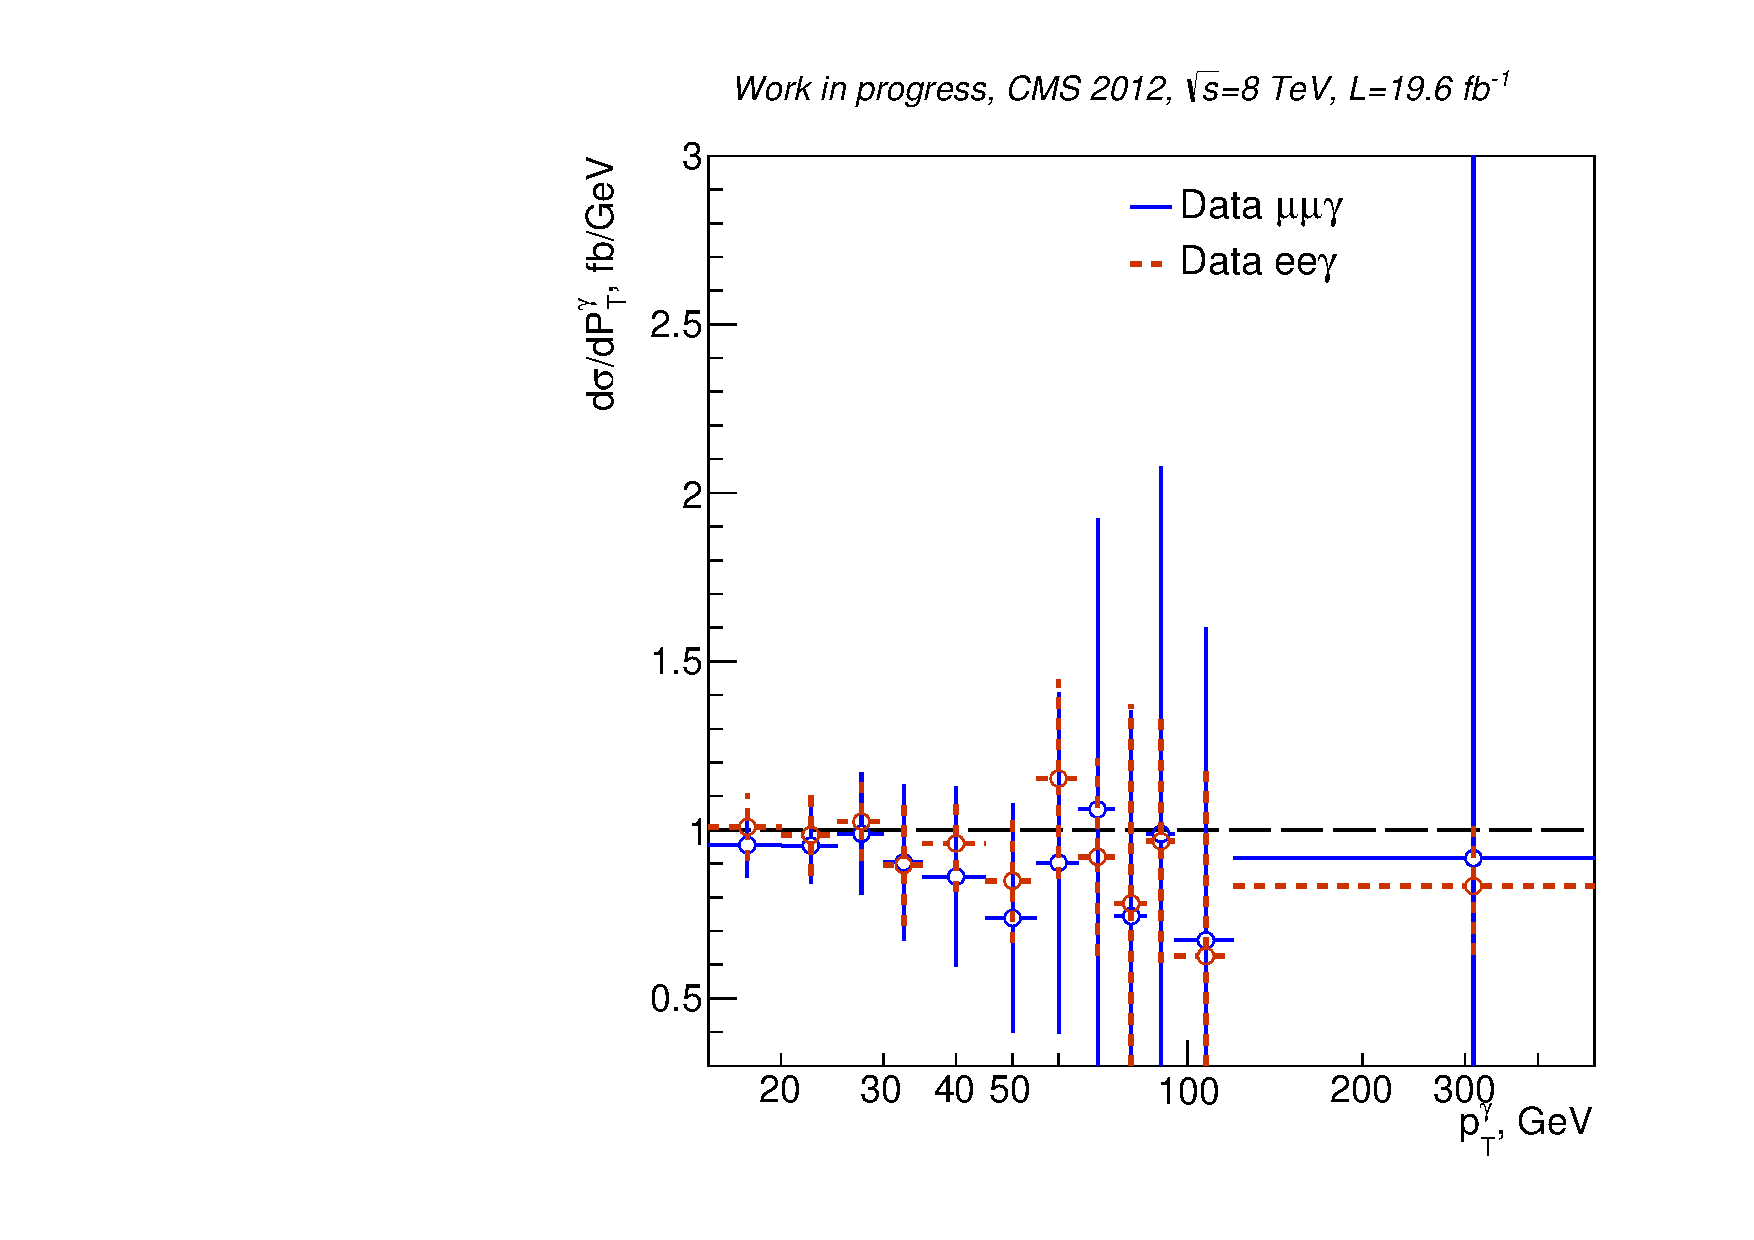
\includegraphics[width=0.45\textwidth]{../figs/figs_v11/ChannelsMERGED_ZGamma/CrossSection/compareCSratioOttoZGamma.pdf}
  \end{center}
\end{figure}
  \tiny
  \begin{itemize}
     \item Double-mu and double-ele datasets are used to perform the Z$\gamma$ check (the same samples as used to prepare templates for jets$\rightarrow\gamma$ background estimation)
     \item Total and differential cross section of Z$\gamma\rightarrowll\gamma$ is measured and compared to the 8 TeV published CMS result
     \item The workflow for Z$\gamma$ is the same as W$\gamma$ except different selection criteria and also Z$\gamma$ has only jets$\rightarrow\gamma$ background
     \item For the muon channel, templates significantly overlay with the dataset, so, the result for the muon channel is a closure test rather that an actual measurement
     \item For the electron channel, templates and dataset are independent
     \item Intermediate plots are available in the AN (template fits, yields, data vs MC)
     \item The result agrees well with the 8 TeV published CMS result
  \end{itemize}
\end{frame}%{Differential Cross Section. Plots}
